\section{Environment and Agent}
\label{sec:Environment and Agent}

The environment for Starcraft 2 to is notoriously complicated, where taken at its raw value the action space would have up to $10^{26}$ per step. Obviously that is computationally to expensive, so there was an environment developed to limit the steps possible. This
can be done with several different thought process combined. One, not all actions that are possible for a given state, are possible for every given state. For example, training a marine without the barracks selected, or even without a barracks built. So that 
can limit action spaces. Another limitation is to combine certain actions, for example selecting marines and attack-moving the units to a different location as a single action instead of 3-4 or more. This is done by reducing actions a using an auto-regressive
chain rule to limit the action space given the context above\cite{starcraft_unplugged}: $$\pi_{\theta}(a|s) = \prod\limits_{l=0}^{L} \pi_{\theta}(a^l|a^{<l}, s)$$.

Another key component to the environment is that Starcraft is an incomplete information game, meaning that there is limited information on the model at any given time, so part of the action space and model needs to learn how to explore and make decision with
incomplete information. 

The agents often have to make use of learning the actions provided in the environment, especially with the capability of so many actions being available at once in the policy. The learning algorithm with seemingly the best results, according to the creators of
pysc2 is, in order of policy gradient, value estimation gradient, and entropy regularisation: 
$$\underbrace{(G_t - v_\theta(s_t))  \nabla_\theta \log \pi_\theta(a_t|s_t)} + \beta \underbrace{(G_t - v\theta(s_t)) \nabla_\theta v_\theta(s_t)} + \eta \underbrace{\sum_a \pi\theta(a|s_t) \log \pi_\theta(a|s_t)}, \qquad (1)$$

While these are the two major equations that go into this environment and recommended agent, they are not the only ones and for more details, refer to the original cited papers. The goal of the agent here is not to match the performance of the previous research
but take the idea of RL in Starcraft II and games in general and aim for a model that can challenge any player, but not aim to win rather then just be challenging.
\subsection{Experiment Details}

With this in mind, the intention of this experiment is not to have the most accomplished Starcraft Model. There have been teams of people, each much more accomplished then myself working on that, but instead to create a model that can fluctuate its
skill with the state of the game. This agent and environment will be run on a machine leaning towards the weak side, running an Nvidia 2070 GPU, 32gbs of ram, and an Intel I7. Tests were run on two machines with the only difference being a 6th gen I7 vs a 10th gen.
These limitations prevents a few advanced features such as using several models to categorize actions with a selection model to chose which action category to take, this experiment will only be using a singular model. Another advanced feature that would in theory
be beneficial for this experiment is to train and use computer vision on replays of professional Starcraft II players, but again due to constraints this will be a simple pure reinforcement learning model. Lastly, the environment will be stripped down, from the
aformentioned details above, with the constraints previously mentioned, a pure environment cannot be used. Instead, it is stripped to 21 different states based on the resources, whats been built, and what units are available. From that state, there are 6 possible
actions. These actions are: do nothing, build supply depot, build barracks, train marines, and attack.  To train, the environment will consist of one agent and a random agent, the experiment will be similar except the opposing agent will differ. Below is an 
image from the environment running.

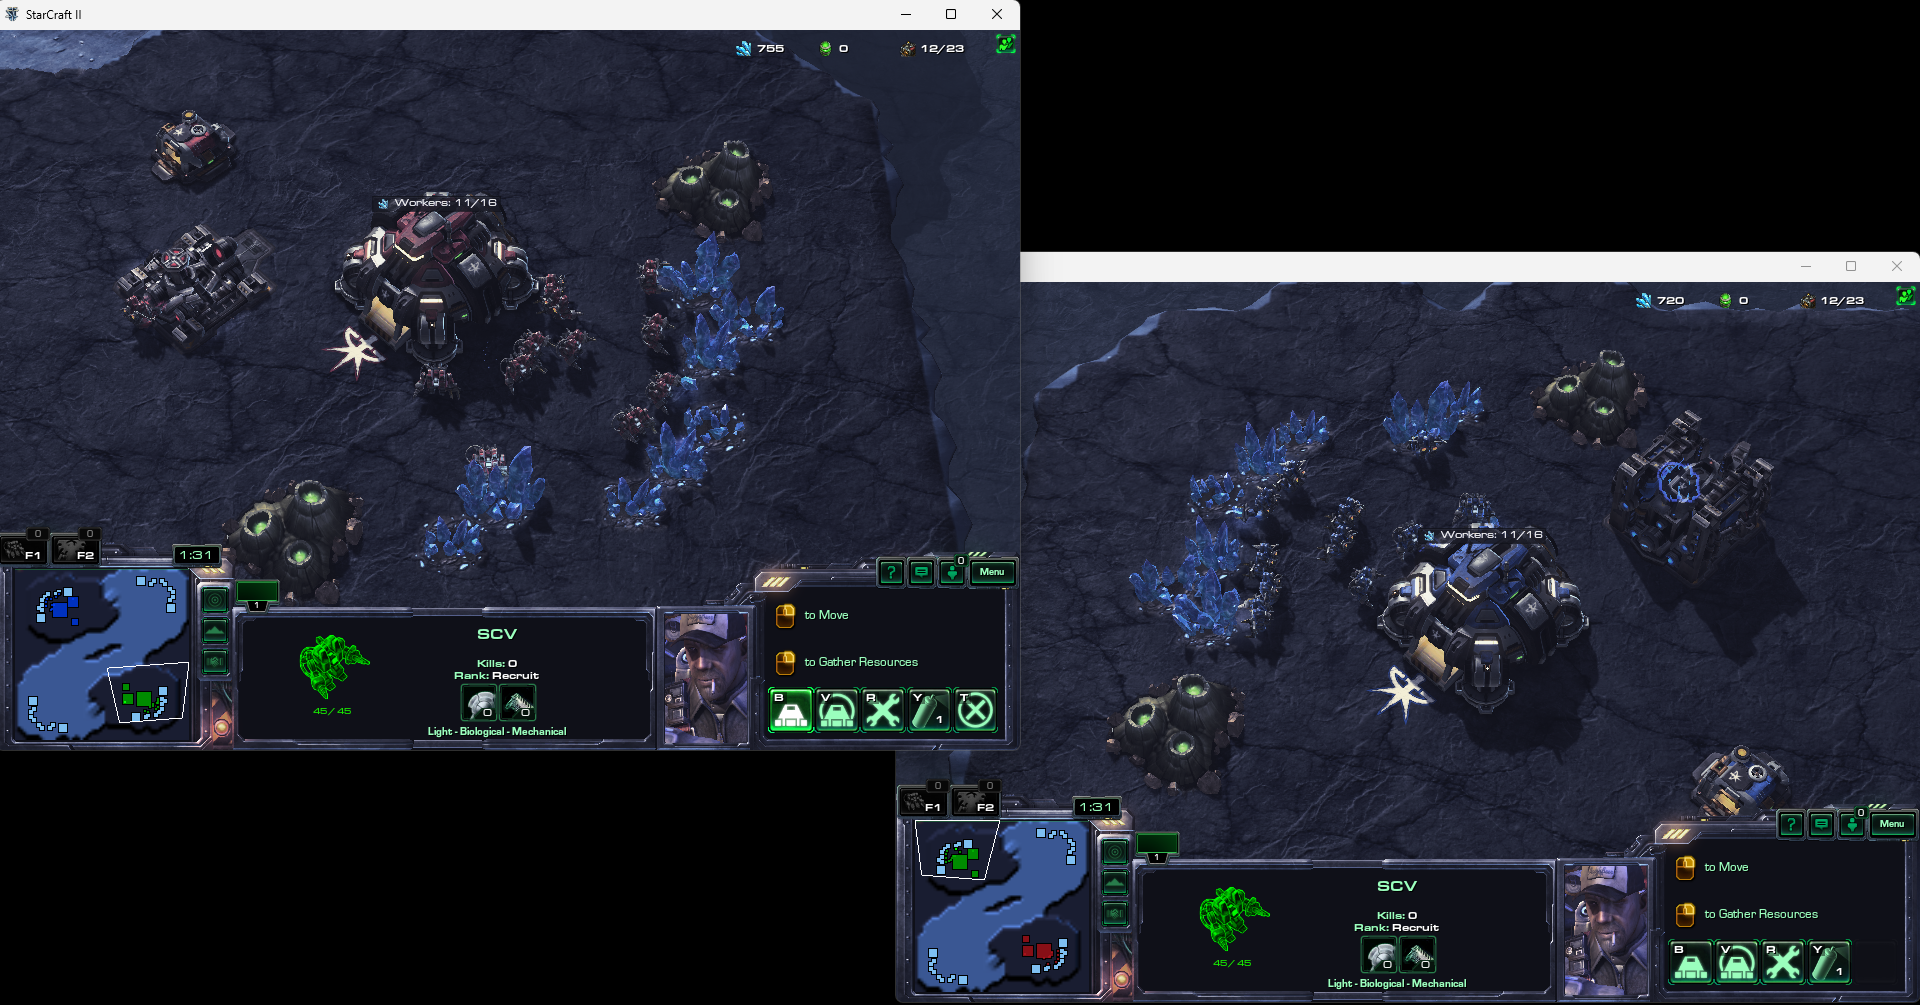
\includegraphics[width=.5\textwidth]{images/sc2env.png}
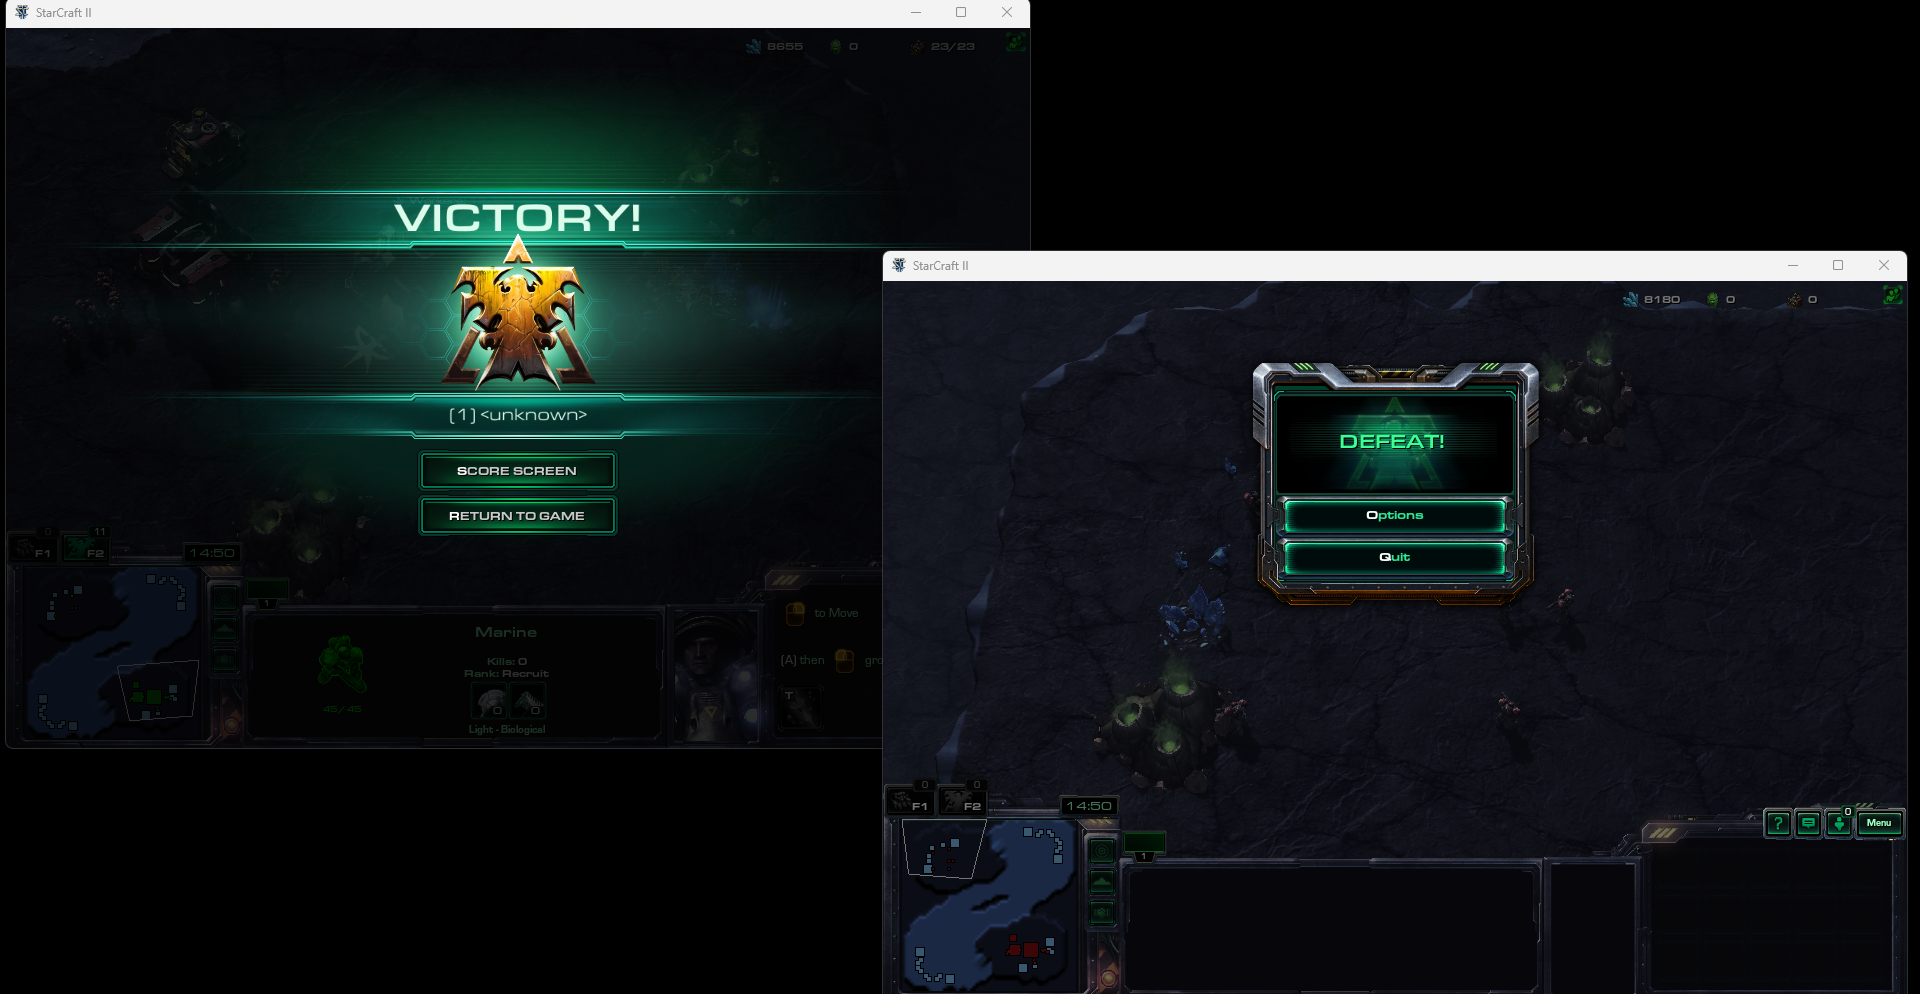
\includegraphics[width=.5\textwidth]{images/victory_screen.png}

\subsection{Agent Details}
Due to the shrunken environment the agents will be fairly limited in their capability as this is not a fully fledged game of Starcraft II. There will be three primary agents in it however, and two are modified to perform this experiment. First, a Q Learning
agent (QL). This is meant to be a reliable, strong, but not perfect model. The adjustments made in order to test the hypothesis have several modes to see what is most likely to give the end goal. There are five action types, normal or none, neutral action to grab
the action in the middle, second for the second best action, quarter for the third-quarter best action, and half best for the half best positive action. Then in addition to that change, in order to implement further tests, there is an alternating variable
to incorporate experiment. Essentially this change has the models action selection alternate from the previous adjustments mention, and the best action that is typical. In essence making half the decisions the best decisions possible, and the other half the 
specified test The second model is a Deep Q Learning agent (DQN). The agent has been implemented with 2 networks in order to stabilize and regularize the agent as it learns. There needs to be a disclaimer with this experiment using these agents. 
Since the environment is simplistic as it is, there could be a missed opportunity to truly test the potential of these changes. More information will be described in future work.

This means that the experiment will be run this way. A player one will be selected from the DQN and QL model. Next a player two will be selected from DQN, QL, and random agent. Player one will have a combination of alternation between the competitive level 
variable, or not, and the combination variable determining the test. As it has been said before, this experiment is not focused on a perfect model, others have done that. The novelty of this experiment is to make a model that can adjust its difficulty based 
on the skill of the opponent, and with three levels of agents here, the experiment should should any measure of success in the theory. 